\documentclass[a4paper,UTF8]{ctexart}
\usepackage{graphicx}
\usepackage{geometry}
\usepackage{xcolor}
\usepackage{amsmath}
\usepackage{enumerate}
\usepackage{caption}
\usepackage{listings}
\usepackage{array}
\usepackage{booktabs}
\usepackage{tikz}
\usetikzlibrary{shapes,arrows}
% \usepackage{pgfplots}
% \pgfplotsset{compat=1.17}
\usepackage{appendix}
\captionsetup[lstlisting]{labelfont=bf,justification=justified}
\usepackage{multicol}
\setlength{\columnsep}{3em}
\usepackage{float}
\usepackage{circuitikz}
\usepackage{ulem}

\graphicspath{{img/}}

\usepackage[colorlinks]{hyperref}
\usepackage{bookmark}
\providecommand{\code}[2]{\lstinputlisting[language=#2,caption=\href{run:#1}{\ttfamily #1},basicstyle=\scriptsize\ttfamily]{#1}}
\providecommand{\img}[1]{\includegraphics[width=0.88\textwidth]{#1}}

% listings
\definecolor{grey}{rgb}{0.8,0.8,0.8}
\definecolor{darkgreen}{rgb}{0,0.3,0}
\definecolor{darkblue}{rgb}{0,0,0.3}
\lstset{%
    numbers=left, %行号
    numberstyle=\scriptsize\color{grey},
    showstringspaces=false,
    showspaces=false,%
    tabsize=4,%
    frame=shadowbox,%
    basicstyle={\ttfamily\normalsize},%
    keywordstyle=\color{blue!80!black}\bfseries,%
    identifierstyle=,%
    commentstyle=\color{green!50!blue}\itshape,%
    stringstyle=\color{green!50!black},%
    rulesepcolor=\color{gray!20!white},
    breaklines,
    columns=flexible,
    extendedchars=false,
    %mathescape=true,
    language=verilog,
}

\begin{document}
\title{\normalsize \underline{计算机系统结构实验}\\\LARGE 实验 6 报告\\\vspace*{1em}\normalsize 类MIPS多周期流水线处理器的设计与实现}
\author{李子龙\\ 518070910095}
\date{\today}
\maketitle
\tableofcontents
\clearpage

\section{实验目的}

\begin{enumerate}
    \item 理解CPU Pipeline,了解流水线冒险(hazard)及相关性,设计基础流水线CPU
    \item 增加Forwarding机制解决数据竞争,减少因数据竞争带来的流水线停顿延时,提高流水线处理器性能
    \item 设计支持Stall的流水线CPU。通过检测竞争并插入停顿(Stall)机制解决数据冒险、控制竞争和结构冒险
    \item 通过predict-not-taken或延时转移策略解决控制冒险/竞争,减少控制竞争带来的流水线停顿延时,进一步提高处理器性能
    \item \sout{将CPU支持的指令数量从16条扩充为31条,使处理器功能更加丰富(选做)}
\end{enumerate}

\section{原理实现}

\subsection{基础流水线}
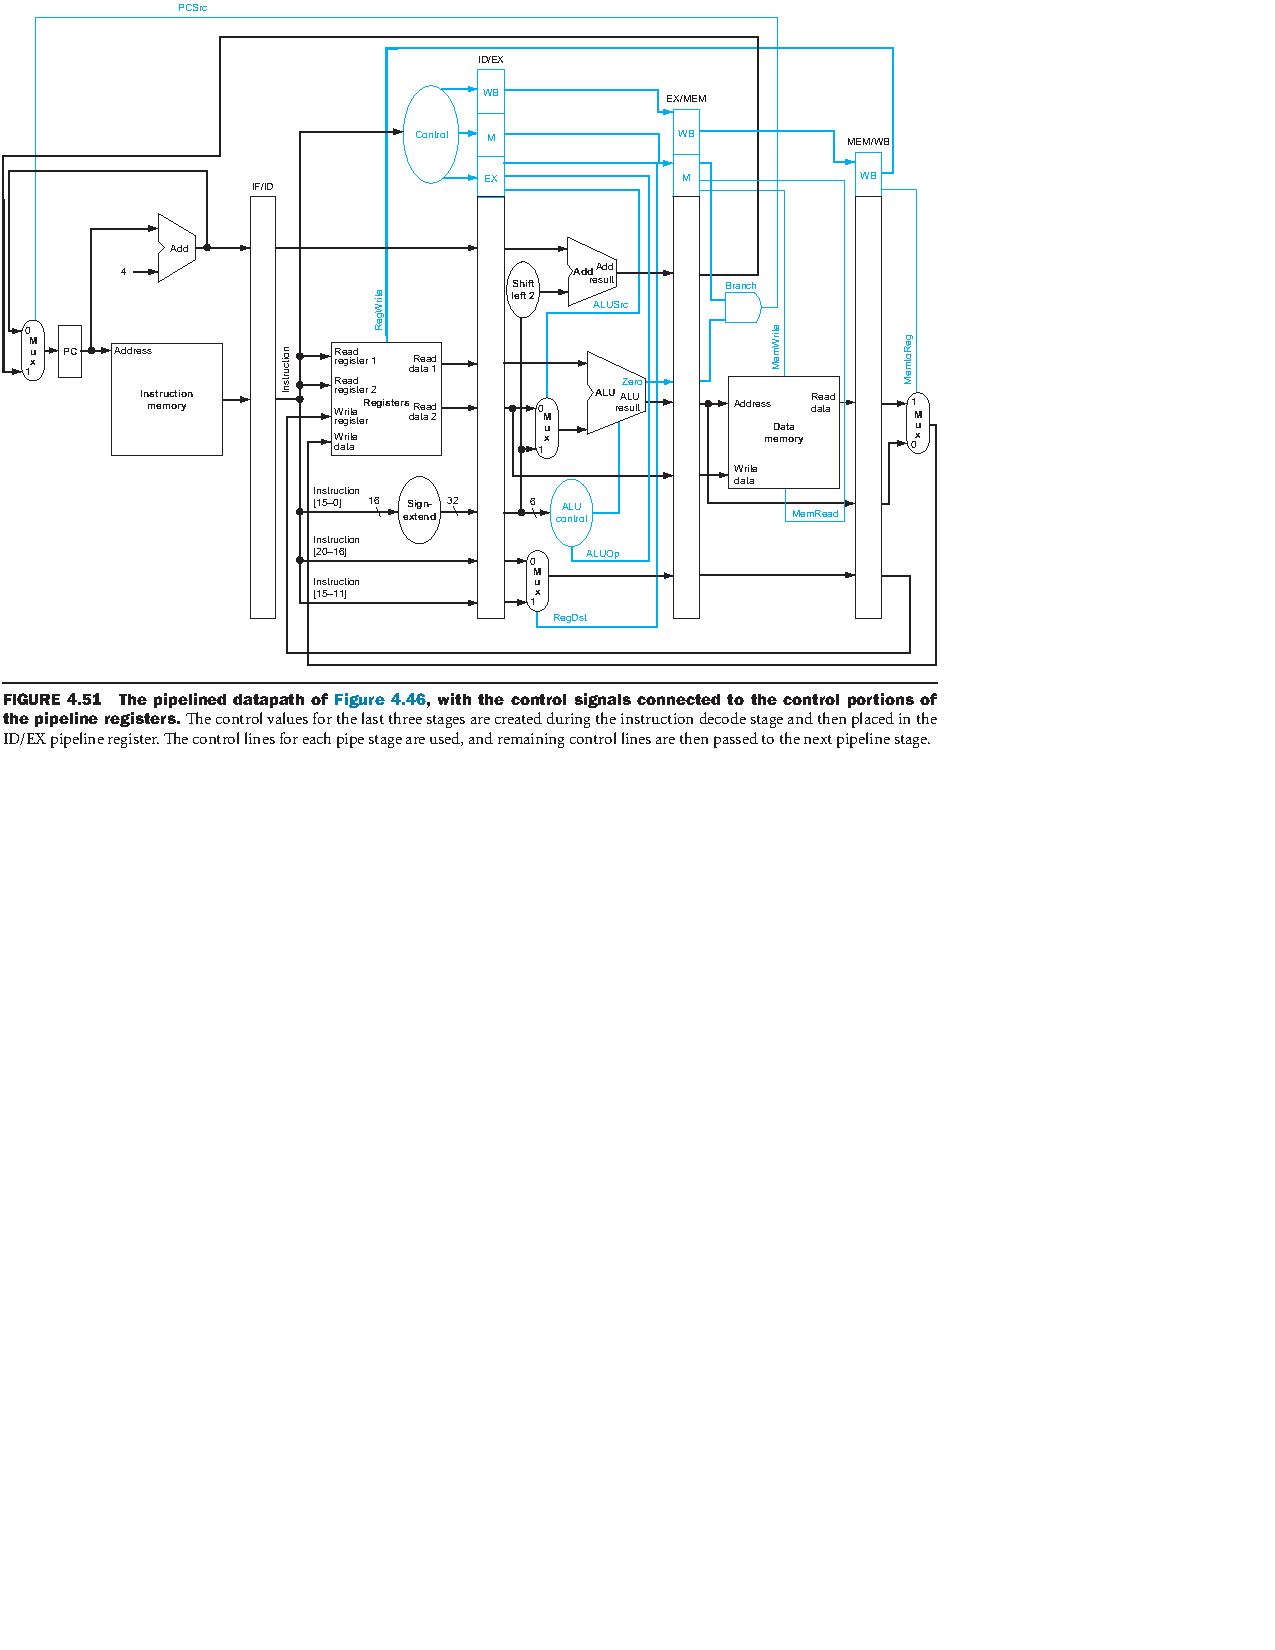
\includegraphics[width=\textwidth]{pipeline.pdf}

通过添加段寄存器,以实现每个阶段的单独运行,并实现流水化。该图是基于 9 条指令的基础流水线设计。基于 16 条指令可以依据实验五进行改造。

\subsection{前向转发机制}\label{sec:fwd}

为了消除数据相关性(比如上一条指令的结果将会作为这一条指令运行),处理器需要引入前向转发机制(Forwarding)。

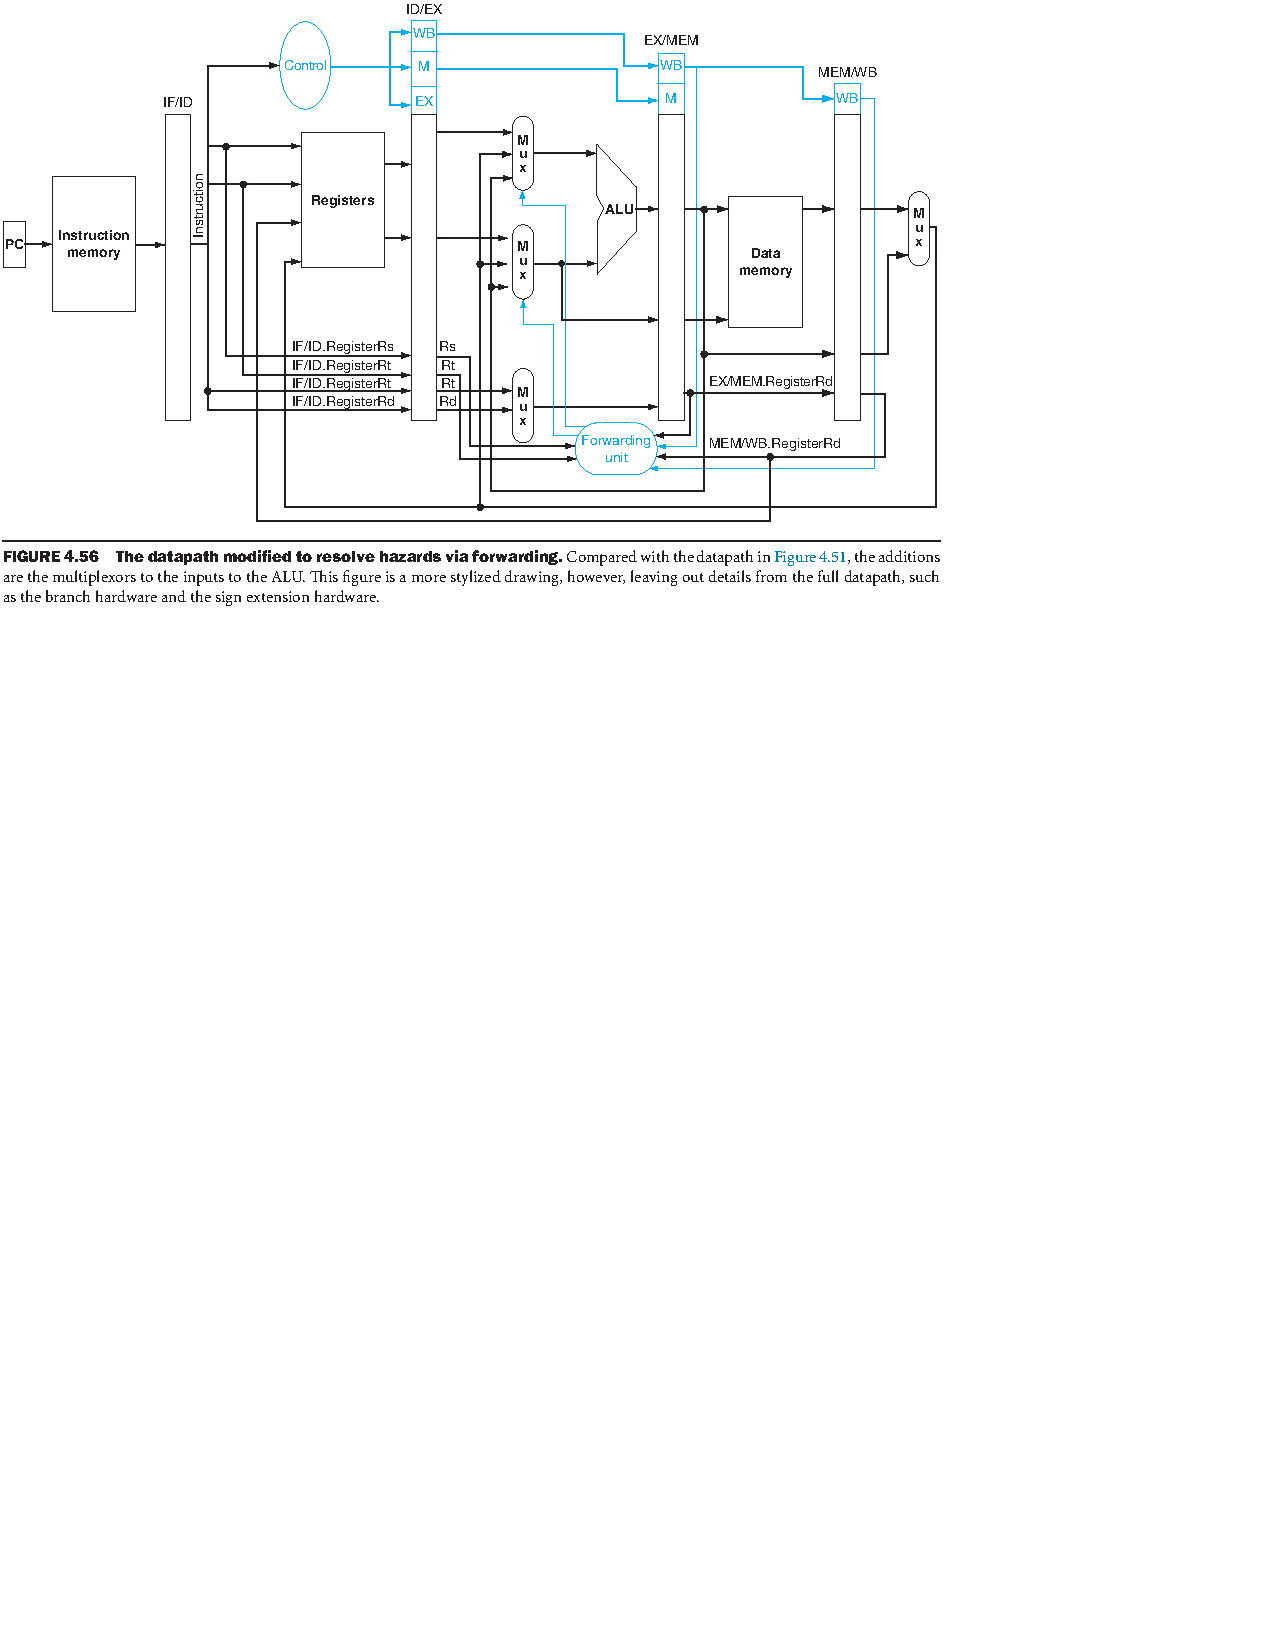
\includegraphics[width=\textwidth]{forwarding.pdf}

\begin{table}[h]
    \centering
    \caption{前向转发机制的控制信号}\label{tab:fwd}
    \begin{tabular}{>{\ttfamily}c>{\ttfamily}ll}
        \toprule
        多选器控制 & 源 & 解释 \\
        \midrule
        ForwardA=00 & ID & 第一个 ALU 操作数来自寄存器堆 \\
        ForwardA=10 & EX & 第一个 ALU 操作数由上一个 ALU 运算结果转发获得 \\
        ForwardA=01 & MEM & 第一个 ALU 操作数从数据存储器或者前面的 ALU 运算结果中转发获得 \\
        ForwardB=00 & ID & 第二个 ALU 操作数来自寄存器堆 \\
        ForwardB=10 & EX & 第二个 ALU 操作数由上一个 ALU 运算结果转发获得 \\
        ForwardB=01 & MEM & 第二个 ALU 操作数由数据存储器或者前面的 ALU 结果转发获得 \\
        \bottomrule
    \end{tabular}
\end{table}

对于两种 EX 冒险 和 MEM 冒险两种模式,根据表 \ref{tab:fwd} 采用以下的判定方法以及输出方式。

\begin{lstlisting}
    wire [1:0] ForwardA = ((EX_REG_WRITE & 
        (EX_WRITE_REG != 0) & 
        (EX_WRITE_REG == ID_INST[25:21])) ? 
            2'b10 : 
            ((MEM_REG_WRITE & (MEM_WRITE_REG != 0) 
            & (MEM_WRITE_REG == ID_INST[25:21])) ? 
                2'b01 : 
                2'b00));
    
    wire [1:0] ForwardB = ((EX_REG_WRITE & 
        (EX_WRITE_REG != 0) & 
        (EX_WRITE_REG == ID_INST[20:16])) ? 
            2'b10 :
            ((MEM_REG_WRITE & (MEM_WRITE_REG != 0) 
            & (MEM_WRITE_REG == ID_INST[20:16])) ? 
                2'b01 : 
                2'b00));

    wire [31:0] ForwardA_RES = 
            ForwardA == 2'b00 ? ID_READ_DATA1 :
                (ForwardA == 2'b10 ? EX_ALU_RES : 
                    WRITE_DATA_WB);
    
    wire [31:0] ForwardB_RES =
            ForwardB == 2'b00 ? ID_READ_DATA2 :
                (ForwardB == 2'b10 ? EX_ALU_RES :
                    WRITE_DATA_WB);
\end{lstlisting}

这样,EX 冒险(10)就可以由 ALU 转发,而 MEM 冒险(01)就可以由写回数据转发。而对于接收者也要做一定的适配,并且为了匹配立即数指令,需要在转发结果后再加选路器。

% EX 冒险:

% \begin{verbatim}
%     if (EX_REG_WRITE && 
%         (EX_WRITE_REG != 0) && 
%         (EX_WRITE_REG == ID_INST[25:21])) 
%         ForwardA = 10;
%     if (EX_REG_WRITE && 
%         (EX_WRITE_REG != 0) && 
%         (EX_WRITE_REG == ID_INST[20:16]))
%         ForwardB = 10;
% \end{verbatim}

% MEM 冒险:

% \begin{verbatim}
%     if (MEM_REG_WRITE && (MEM_WRITE_REG != 0) 
%         && !(EX_REG_WRITE && (EX_WRITE_REG != 0)
%             && (EX_WRITE_REG != ID_INST[25:21]))
%         && (MEM_WRITE_REG == ID_INST[25:21]))
%         ForwardA = 01;
%     if (MEM_REG_WRITE && (MEM_WRITE_REG != 0) 
%         && !(EX_REG_WRITE && (EX_WRITE_REG != 0)
%             && (EX_WRITE_REG != ID_INST[20:16]))
%         && (MEM_WRITE_REG == ID_INST[20:16]))
%         ForwardB = 01;
% \end{verbatim}

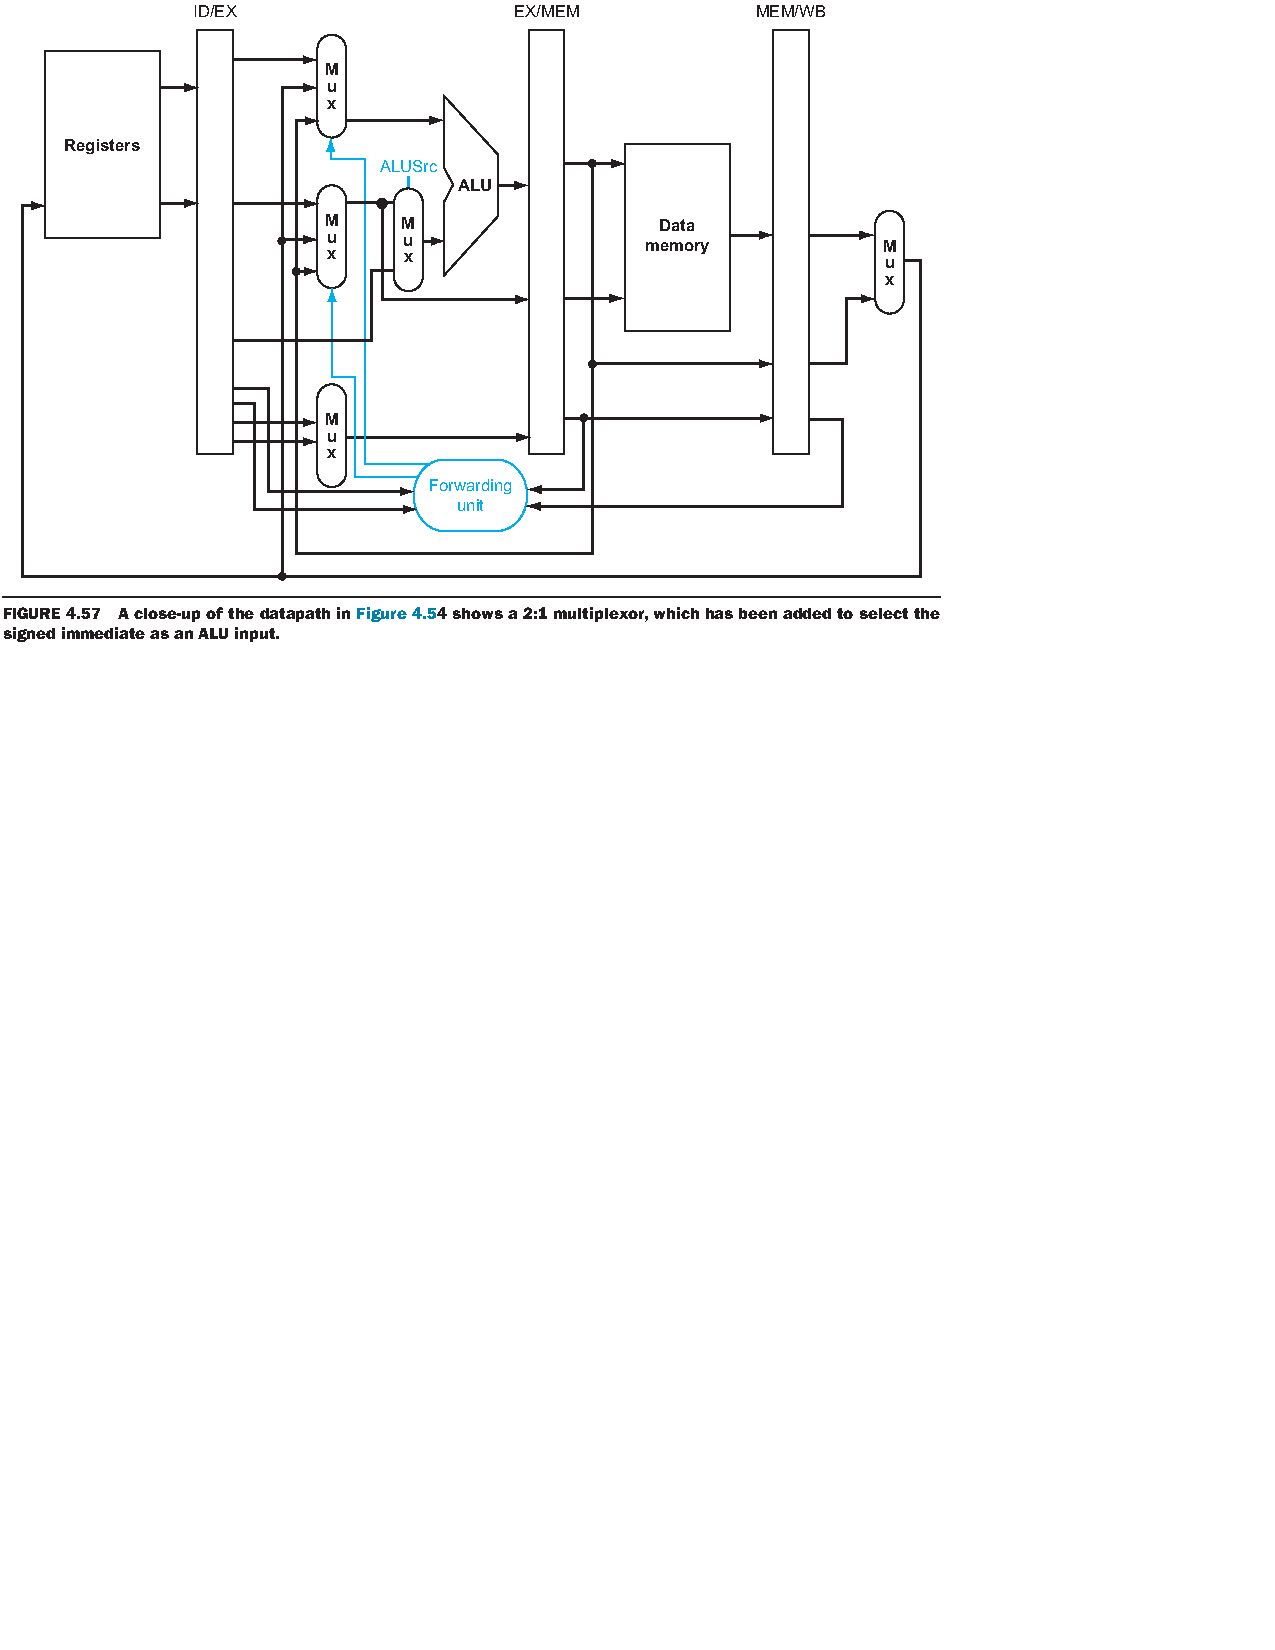
\includegraphics[width=\textwidth]{Imm.pdf}

\begin{lstlisting}
    ALU alu(
        .input1(SHAMT ? ID_INST[10:6] : ForwardA_RES), // ForwardA
        .input2(ID_ALU_SRC ? ID_OPRAND : ForwardB_RES), // ForwardB
        .aluCtr(ALU_CTR),
        .zero(ZERO_EX),
        .aluRes(ALU_RES_EX)
    );
    
    dataMemory DataMemory(
        .Clk(clk),
        .address(EX_ALU_RES),
        .writeData(ForwardB_RES),   // ForwardB
        .memWrite(EX_MEM_WRITE),
        .memRead(EX_MEM_READ),
        .readData(READ_DATA_MEM)
    );
\end{lstlisting}

值得注意的是,存储器的写入数据使用了前向传递B的结果。

并且在 WB 级不会发生冒险的前提是
\begin{quotation}
    假设在 ID 级指令读取的存储器与 WB 级指令写入的寄存器是同一个寄存器时,就由寄存器堆提供正确的结果。
\end{quotation}
因此,寄存器堆的输出不能依赖于输入地址的变化,一旦数据出现了变化,就需要立刻输出更新值。这可以采用 \verb"wire" 类型直接赋值实现,这样一旦时钟下沿写入,就会被立刻更新为新值,从而影响下一时钟上沿的赋值。
% \begin{multicols}{2}
    \code{Registers.v}{verilog}
% \end{multicols}

% \begin{verbatim}
%     ALU alu(
%         .input1(SHAMT ? ID_INST[10:6] : 
%             (ForwardA == 2'b00 ? ID_READ_DATA1 :
%                 (ForwardA == 2'b10 ? EX_ALU_RES : 
%                     WRITE_DATA_WB))
%         ),
%         .input2(ID_ALU_SRC ? ID_OPAND : 
%             (ForwardB == 2'b00 ? ID_READ_DATA2 :
%                 (ForwardB == 2'b10 ? EX_ALU_RES :
%                     WRITE_DATA_WB))
%         ),
%         .aluCtr(ALU_CTR),
%         .zero(ZERO_EX),
%         .aluRes(ALU_RES_EX)
%     );
% \end{verbatim}

\subsection{停顿机制}

当寄存器尚未获得值且紧随的运算需要该寄存器的后值时,仅仅前向转发是不足的。这时候就要引入停顿机制。

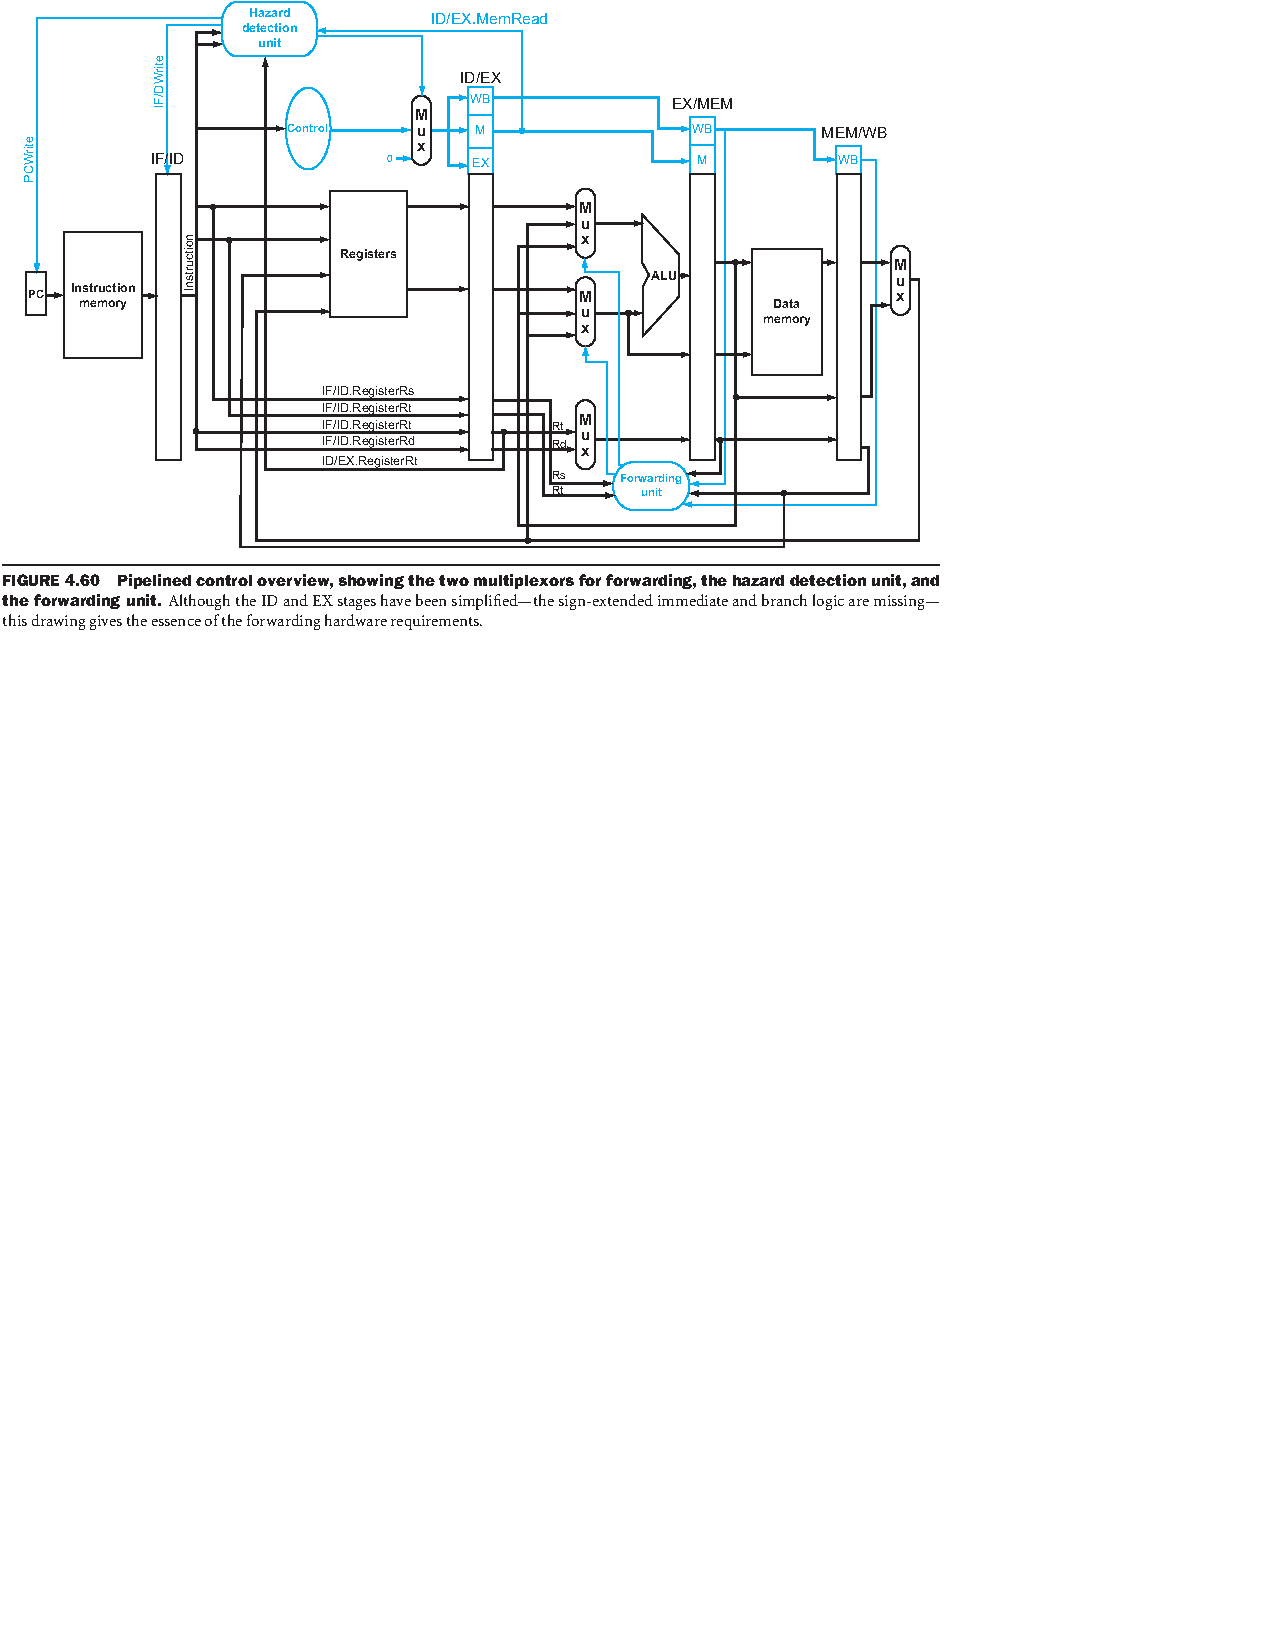
\includegraphics[width=\textwidth]{stall.pdf}

用来解决 lw - use 冒险,就需要考察读取的存储器是不是使用的存储器。

\begin{verbatim}
    wire stalling = (ID_MEM_READ && 
        ((ID_INST[20:16] == IF_INST[25:21]) 
        || (ID_INST[20:16] == IF_INST[20:16]))) ? 
            1 : 0;
\end{verbatim}

一旦停顿机制被激活,就会向流水线中添加一个气泡以停顿,方法就是IF 值被维持和 ID 控制信号清除(这一步预测不发生共用)。

\begin{lstlisting}
    if (stalling || (ID_BRANCH && BEQ)) begin
        // nop
        ID_REG_DST <= 0;
        ID_JUMP <= 0;
        ID_BRANCH <= 0;
        ID_MEM_READ <= 0;
        ID_MEM_TO_REG <= 0;
        ID_MEM_WRITE <= 0;
        ID_ALU_OP <= 0;
        ID_ALU_SRC <= 0;
        ID_IMM <= 0;
        ID_JAL <= 0;
        ID_REG_WRITE <= 0;
    else //...

    // IF
    if(stalling == 0) begin
        PC <= PC + 4;
        IF_PC <= PC;            // Has already been PC + 4
        IF_INST <= INST_IF;
    end // stalling means no change
\end{lstlisting}

\subsection{预测不发生机制}\label{sec:pnt}

最后来处理分支情况。如果采用传统的方式,发生分支时,需要等待分支在 EX 段才可以判断,此前需要一直阻塞(3个周期)。这样做实在太慢,不利于流水线的运转。

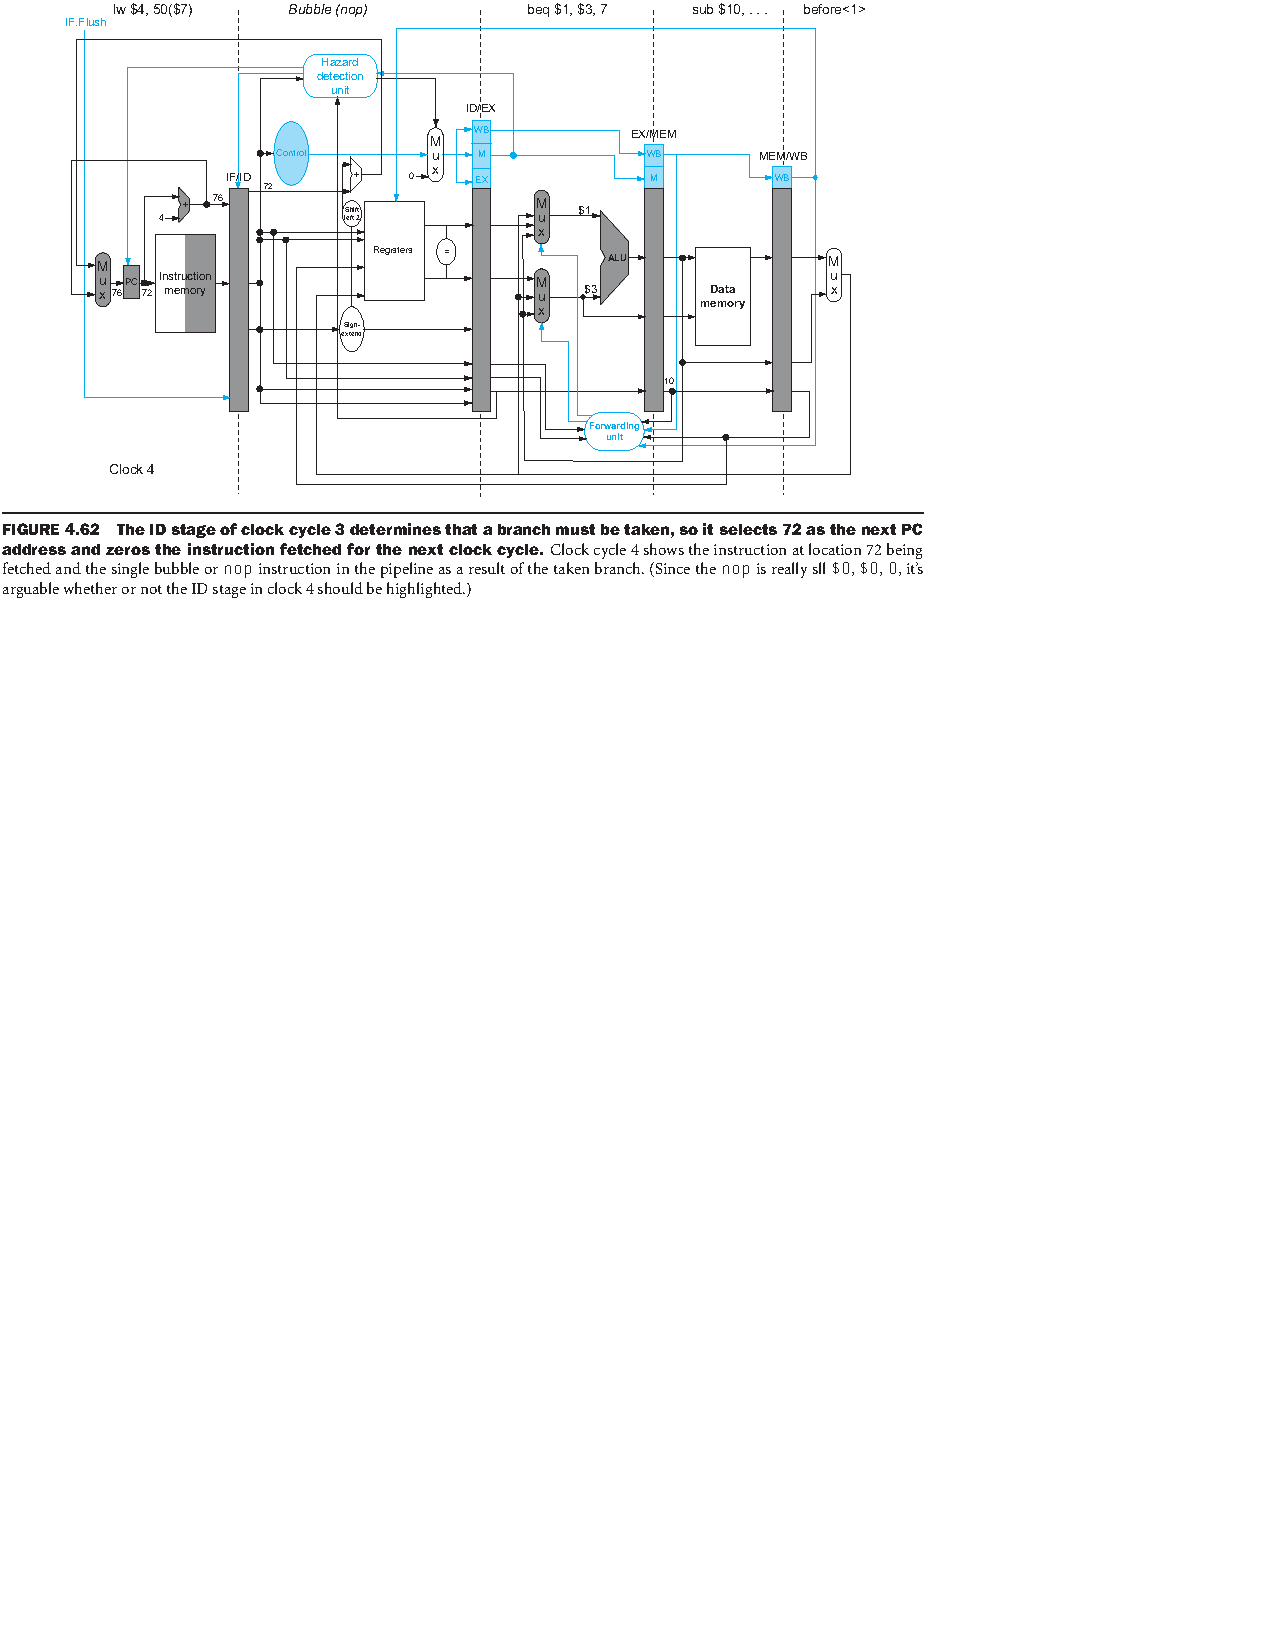
\includegraphics[width=\textwidth]{predict-not-taken.pdf}

仔细阅读课本后,将做如下的设计:遇到分支认为不运行分支,计数器继续递增。而将 branch 判定提前到 ID 段,一旦发现判断错误,就会向流水线中加入一个气泡,并将 PC 设定为分支位置,将IF寄存器清空(IF.Flush)。气泡是在时钟上沿进行(前文已提到),而后面的需要在时钟下沿进行,为了影响后面所有指令的进行(在后文的处理器顶端模块编写中可以看到赋值顺序是从后向前进行的,以传递数据,这样做可以在不影响整个代码风格的情况下,以影响后面的指令,否则只会不会在前面阻塞,后面赋值又会覆盖)。

\begin{lstlisting}
    always @(negedge clk ) begin
        // Here is the clear signal before transition.
        // IF.Flush
        if(ID_BRANCH && BEQ) begin
            PC <= BRANCH_PC_ID;
            IF_PC <= 0;
            IF_INST <= 0;
        end
        //...
    end
\end{lstlisting}

判断的方法需要直接使用前向传递的数据,判定两个操作数是否相等。否则会在特定的事件产生判断错误的结果(比如分支指令前恰好是 ALU 指令,这时必然要阻塞)。

\begin{lstlisting}
    // predict-not-taken
    wire BEQ = (ForwardA_RES == ForwardB_RES);
\end{lstlisting}

\subsection{代码风格与顶端设计}\label{sec:code}

有了上面的考虑之后,就可以进行流水线的顶端设计了。

本处理器的\textbf{代码风格}如下:
\begin{itemize}
    \item 所有的段寄存器都会采用前一阶段的名称作为开始。比如 IF/ID 寄存器中的 INST,就会被定义为
    \begin{lstlisting}
        reg [31:0] IF_INST;
    \end{lstlisting}
    以表示该值由 IF 阶段发出。
    \item 所有的电线采用终止寄存器结尾。比如 IF 阶段的指令存储器发出指令信息以存储到 IF/ID 寄存器,就会被定义下面的方式,表示电线将会在 IF/ID 寄存器终止。
    \begin{lstlisting}
        wire [31:0] INST_IF;
    \end{lstlisting}
    \item 所有段寄存器的值会在时钟上跳沿被逆阶段更新,也就意味着寄存器的值将会晚电线值一个周期。比如
    \begin{lstlisting}
        always @(posedge clk) begin
        // reset
        // WB
        // MEM
        // EX
        // ID
            ID_INST <= IF_INST;
        // IF
            IF_INST <= INST_IF;
        end
    \end{lstlisting}
    这样做就可以防止不确定的赋值顺序。当需要实时值时需要使用以阶段结尾的电线值(一般在时钟沿之外使用),在时钟沿更新时如果没有对应的直接输出电线,就要采用寄存器值更新。
    \item 当需要影响全阶段的运行时,需要在时钟下沿更新值。这一点与实验五的设计是一致的。比如跳转(含 JR 指令)、分支指令判断错误等:
    \begin{lstlisting}
    always @(negedge clk ) begin
        // IF.Flush
        if(ID_BRANCH && BEQ) begin
            PC <= BRANCH_PC_ID;
            IF_PC <= 0;
            IF_INST <= 0;
        end
        if(EX_JR) begin
            PC <= EX_ALU_RES;
            IF_PC <= 0;
            IF_INST <= 0;
            ID_PC <= 0;
            ID_INST <= 0;
            ID_REG_DST <= 0;
            ID_JUMP <= 0;
            ID_BRANCH <= 0;
            ID_MEM_READ <= 0;
            ID_MEM_TO_REG <= 0;
            ID_MEM_WRITE <= 0;
            ID_ALU_OP <= 0;
            ID_ALU_SRC <= 0;
            ID_IMM <= 0;
            ID_JAL <= 0;
            ID_REG_WRITE <= 0;
        end else
            PC <= EX_JUMP ? EX_JUMP_PC : PC;
    end
    \end{lstlisting}
\end{itemize}

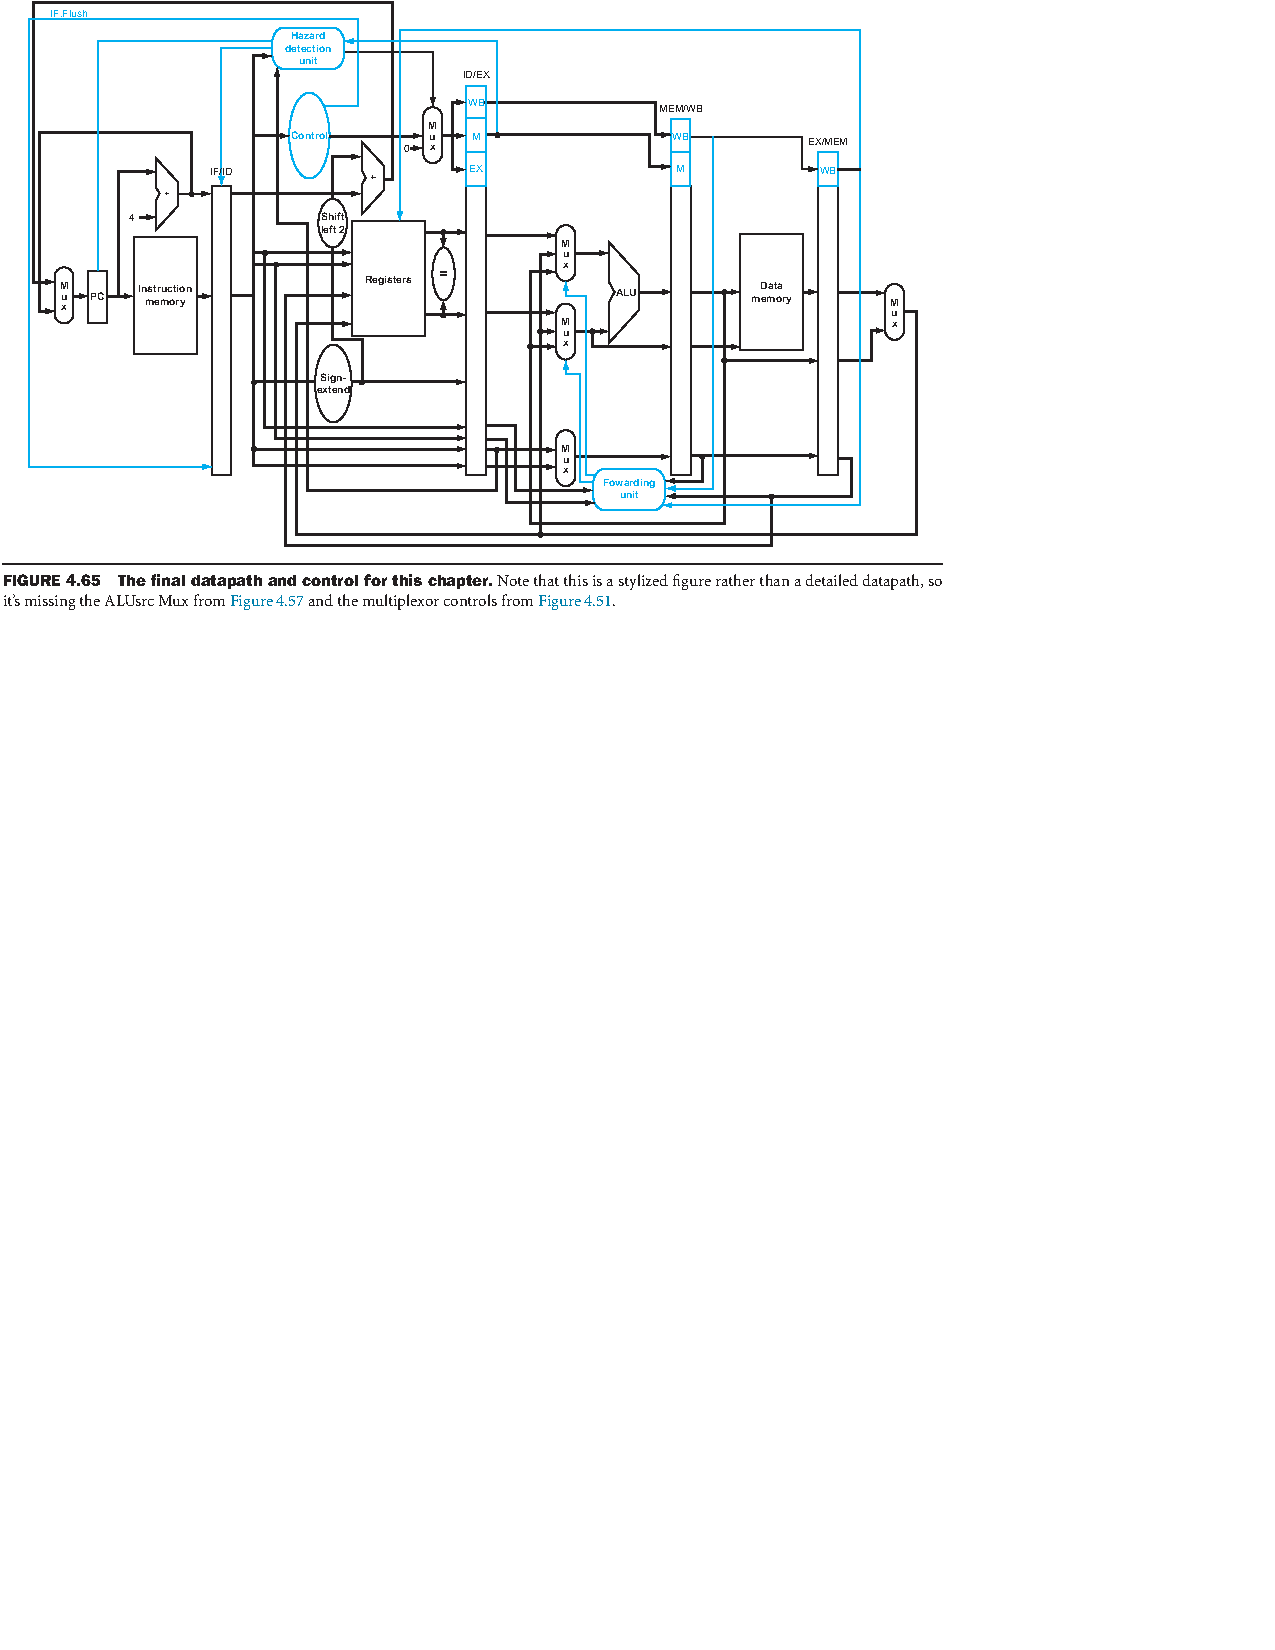
\includegraphics[width=\textwidth]{FINAL.pdf}

\begin{multicols}{2}
    \code{Top.v}{verilog}
\end{multicols}

\section{仿真结果}

\subsection{思考问题}

在完成实现后,先回答一些思考题目。
\begin{enumerate}
    \item 请思考和Lab5相比,Top模块中的主要变化处是什么?\par
    \textbf{答} 需要考虑赋值的顺序,不能像 Lab 5 一样将电线直接接上。更重要的是,需要考虑冒险问题。
    \item 之前的模块是否要修改?\par
    \textbf{答} 需要修改,比如 Registers 的相关修改,见 \ref{sec:fwd}。
    \item 另外,由于MEM级的Branch会影响PCSrc的值,从而影响下次PC,因此需要为Control加入RESET功能,将Branch置零。\par
    \textbf{答} 该问题在预测不发生机制统一考虑,见 \ref{sec:pnt}。
    \item 由于各种变量名称极为复杂,推荐在着手编码之前为自己选择一套命名规范\par
    \textbf{答} 见代码风格 \ref{sec:code}。
    \item 在实现实验目的2.,3.,4.的内容时建议把1.的代码或工程备份一遍才开始\par
    \textbf{答} 本实验采用 git 版本控制工具统一管理。
\end{enumerate}

\subsection{Mars 汇编程序}

为了加快测试进度,在本实验中采用计算机结构理论课上的 Mars 工具快速生成汇编二进制代码。

打开 Mars。新建 asm 汇编程序,然后汇编后,在文件选单中 Dump Memory,另存为 Binary Text 就可以生成二进制程序码。值得注意的是,需要采用标签指定 beq 的目标位置,也就是实验指导书中的示例汇编代码风格。

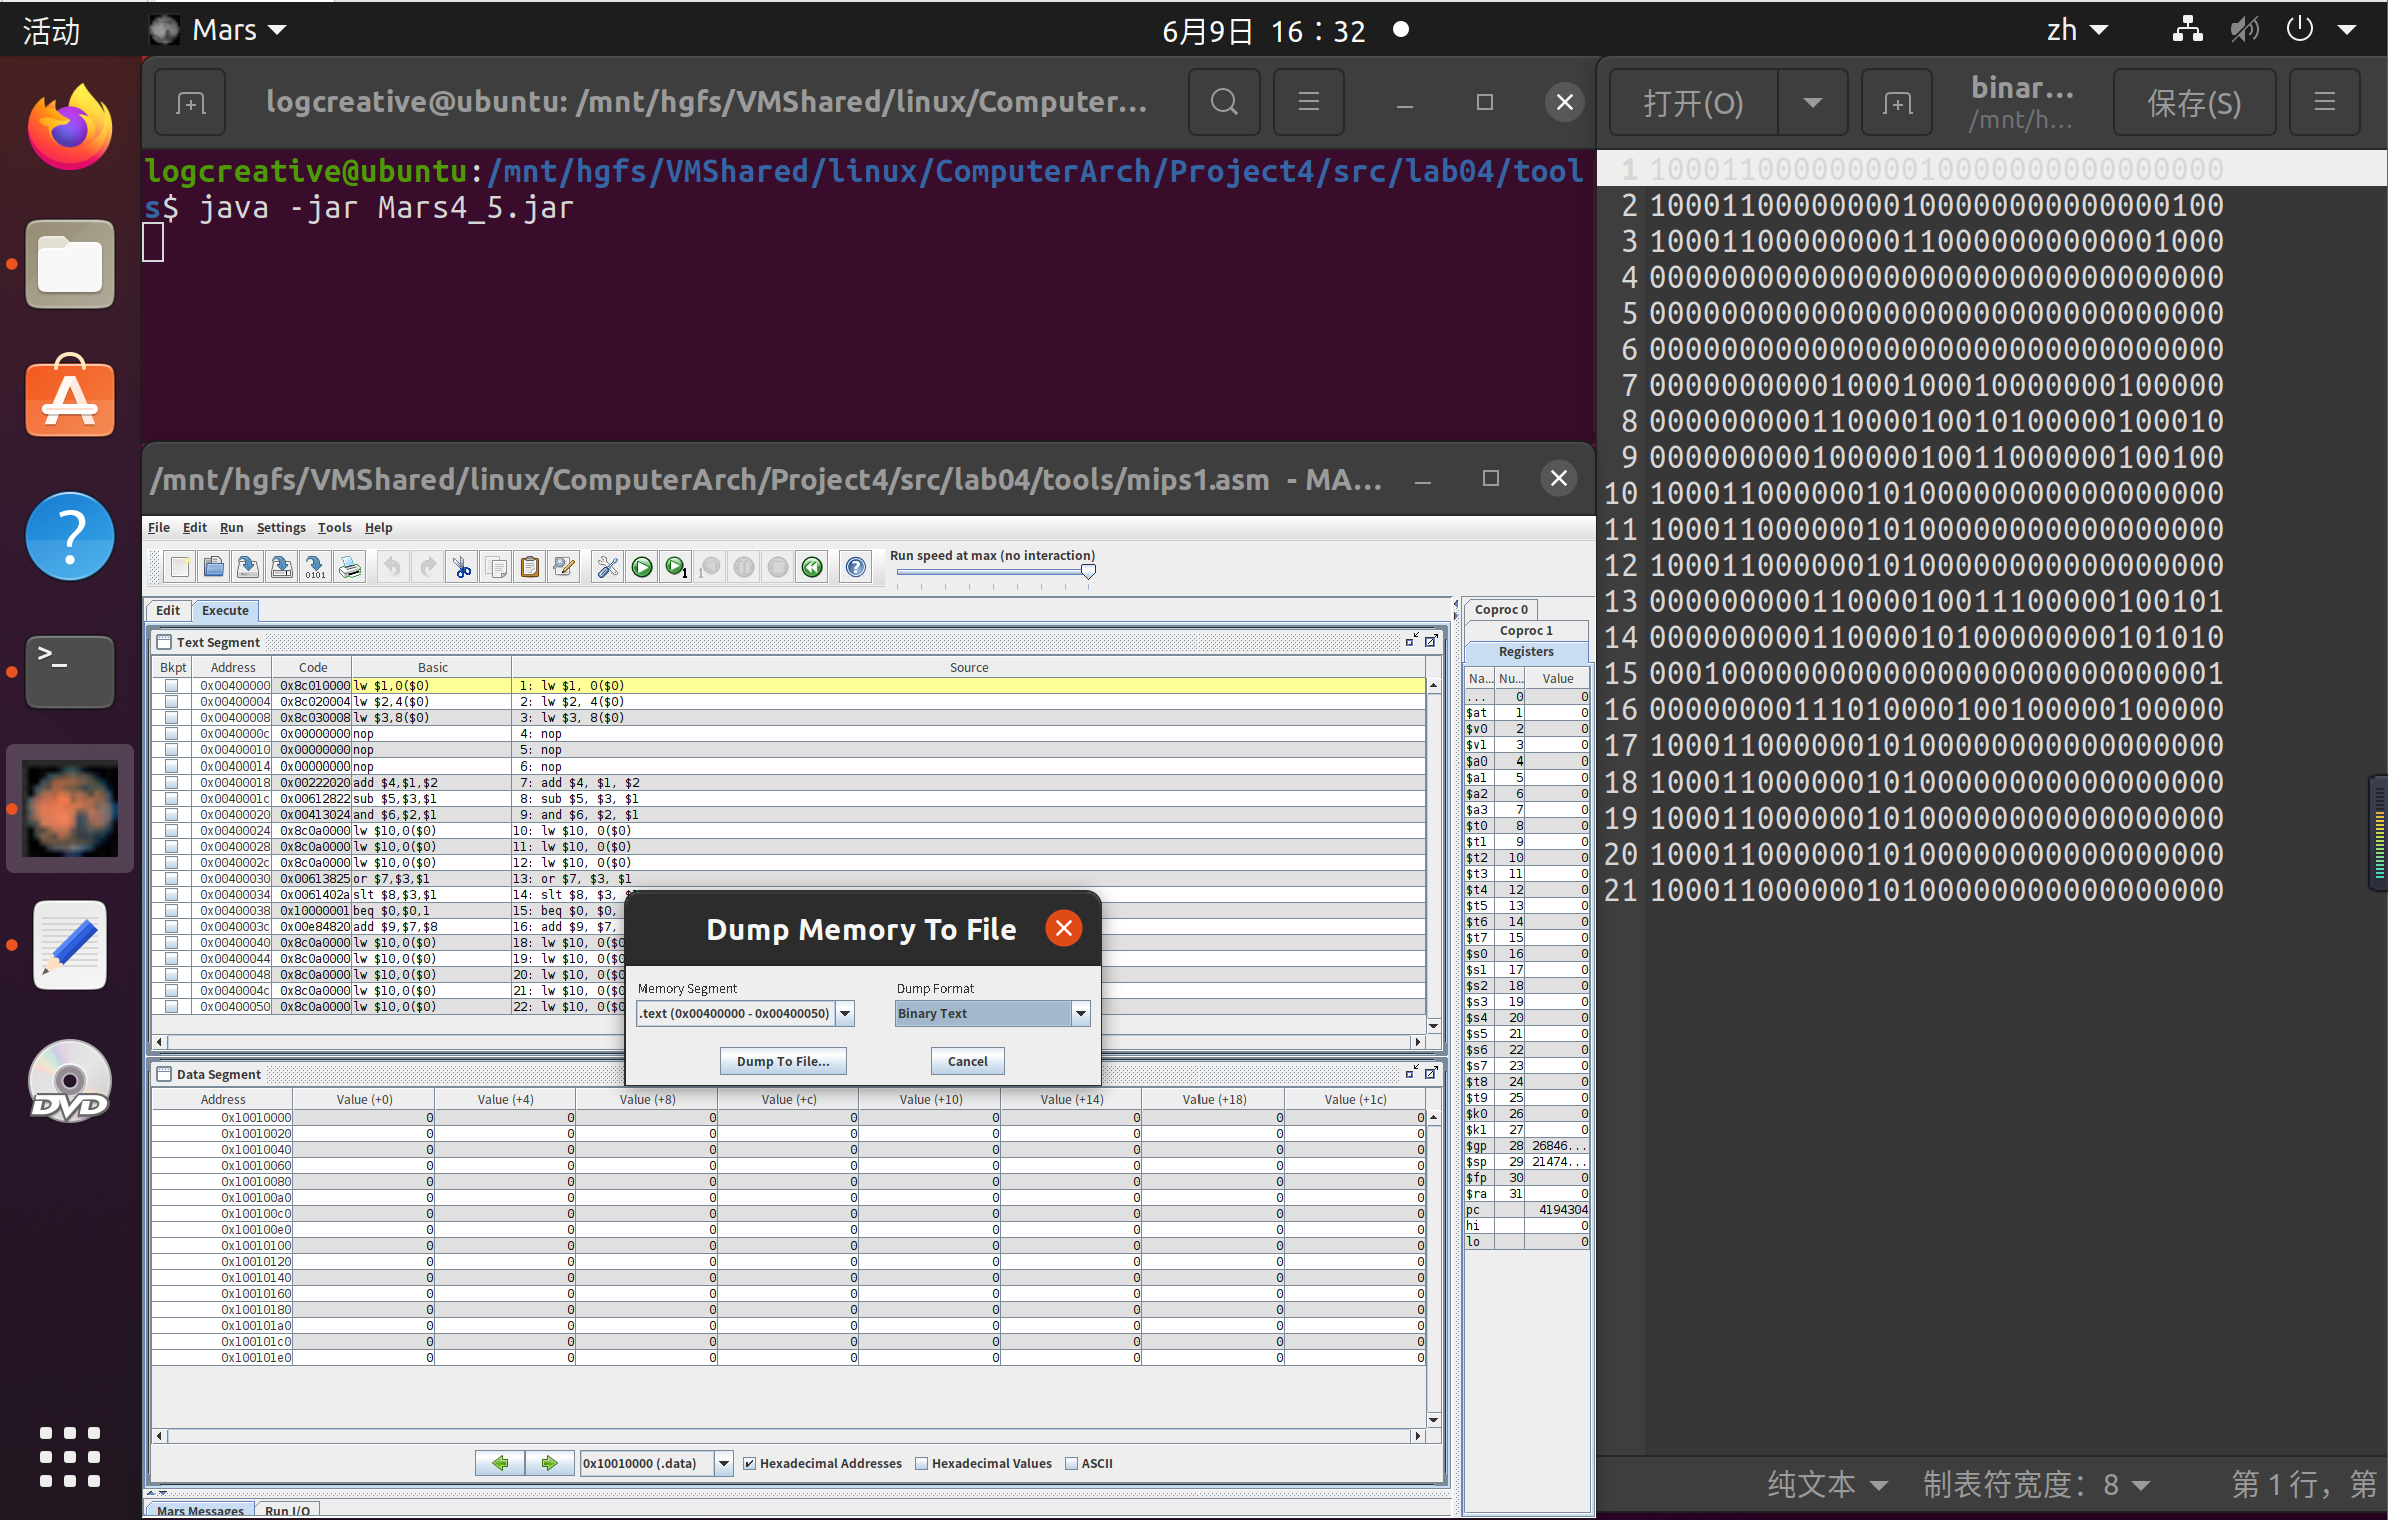
\includegraphics[width=\textwidth]{mars.png}

\subsection{无优化仿真}

首先采用教材代码,然后会有数据冒险问题。

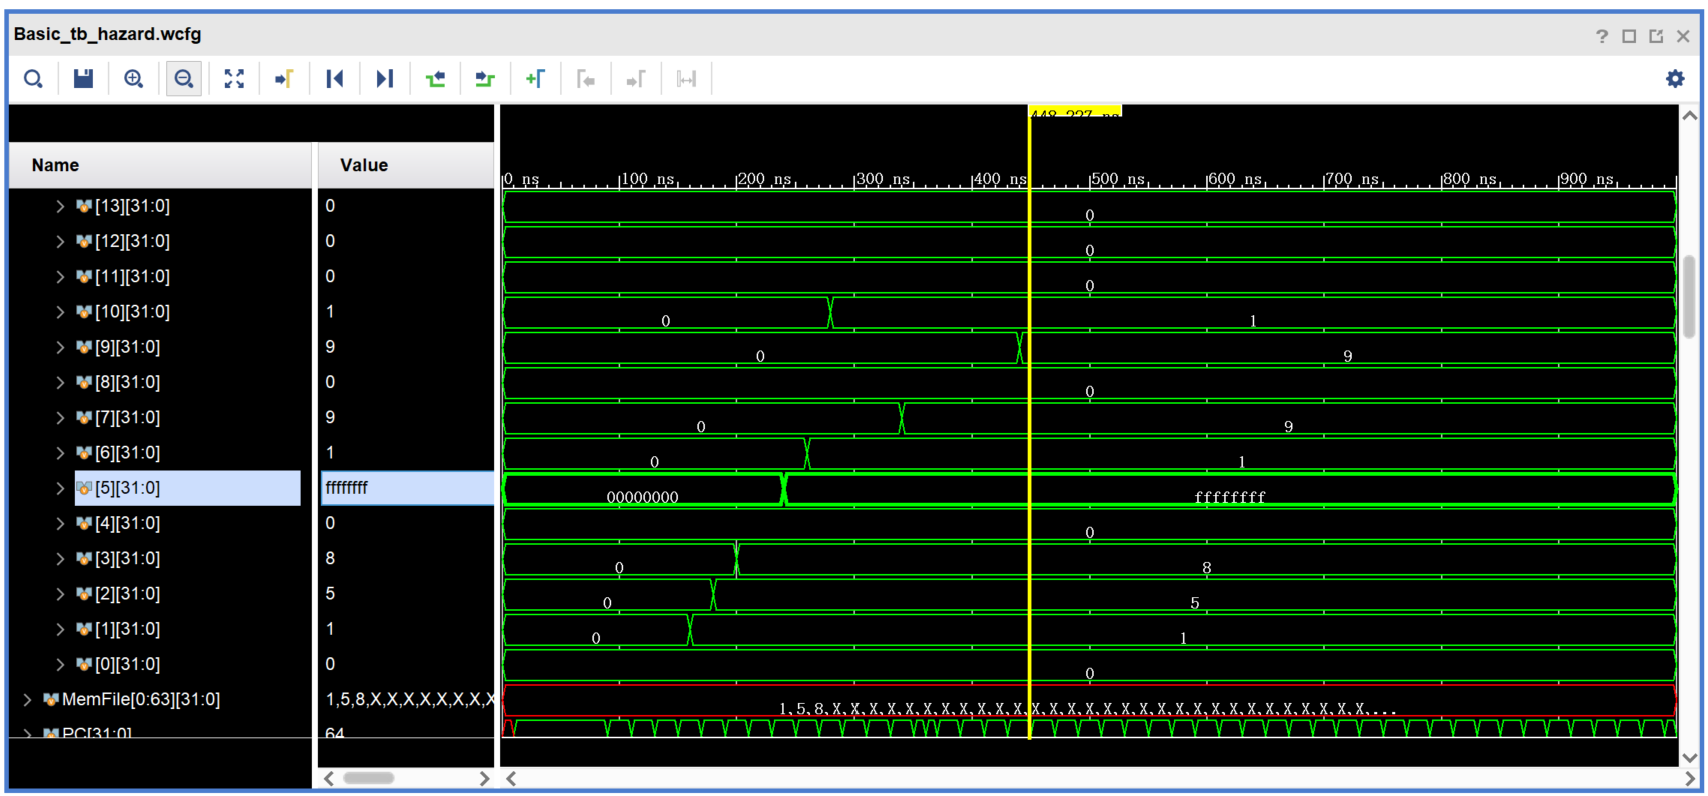
\includegraphics[width=\textwidth]{hazard.png}

手动插入空语句后(lw-use型需要三个空语句),就可以解决数据冒险问题。从而得到预期结果。

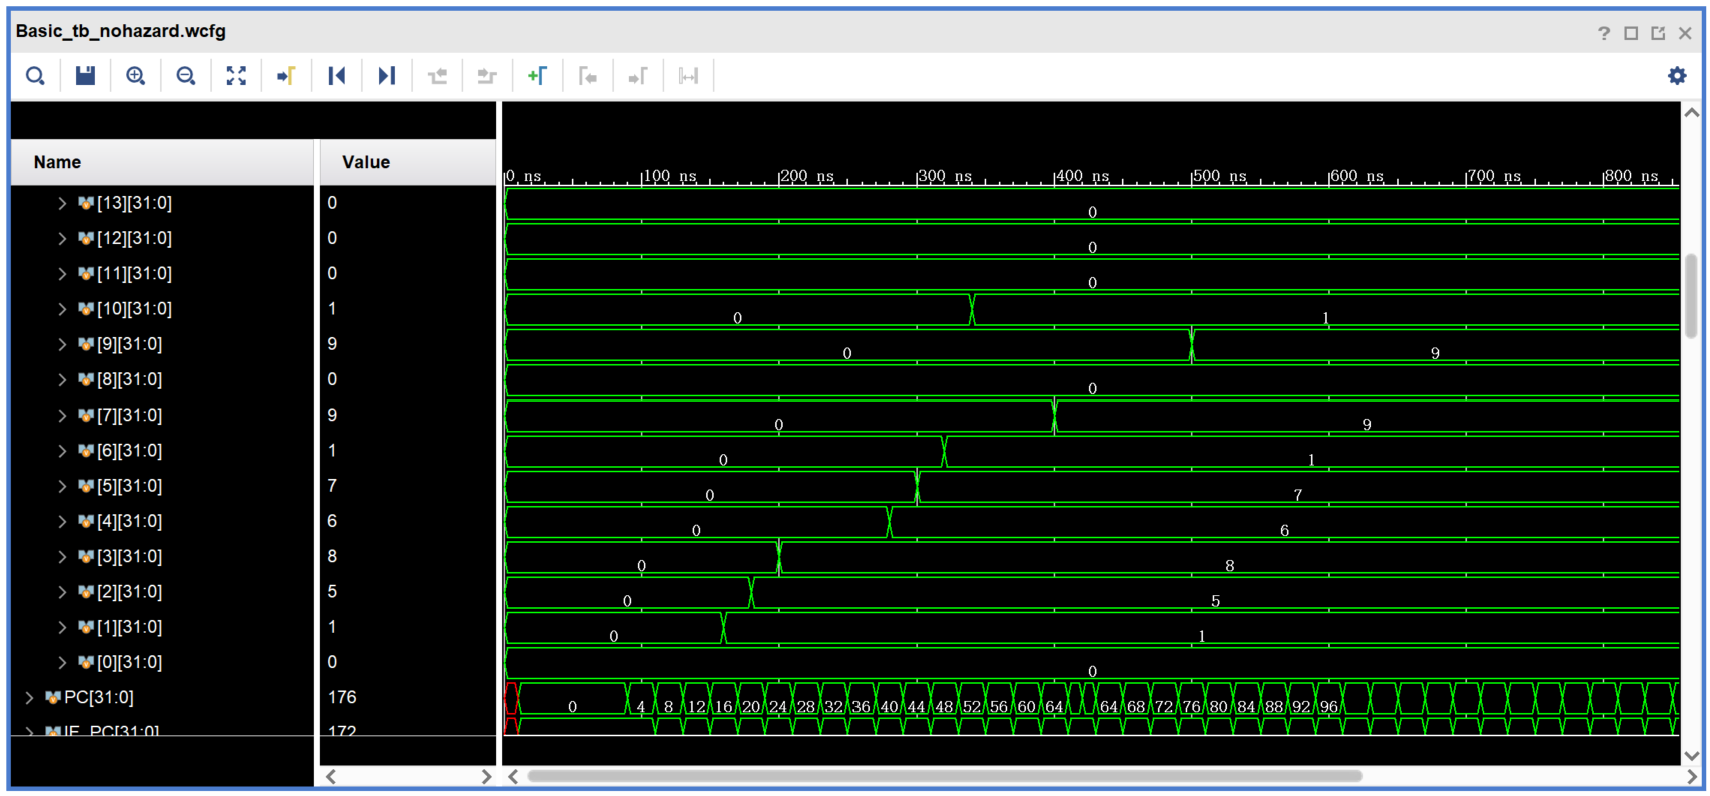
\includegraphics[width=\textwidth]{nohazard.png}

\begin{multicols}{2}
    \begin{lstlisting}[caption=example.asm]
lw $1, 0($0)
lw $2, 4($0)
lw $3, 8($0)
add $4, $1, $2
sub $5, $3, $1
and $6, $2, $1
lw $10, 0($0)
lw $10, 0($0)
lw $10, 0($0)
or $7, $3, $1
slt $8, $3, $1
beq $0, $0, end
add $9, $7, $8
end:lw $10, 0($0)
lw $10, 0($0)
lw $10, 0($0)
lw $10, 0($0)
lw $10, 0($0)
    \end{lstlisting}
\vskip4em
    \begin{lstlisting}[caption=example.asm(no risk)]
lw $1, 0($0)
lw $2, 4($0)
lw $3, 8($0)
nop
nop
nop
add $4, $1, $2
sub $5, $3, $1
and $6, $2, $1
lw $10, 0($0)
lw $10, 0($0)
lw $10, 0($0)
or $7, $3, $1
slt $8, $3, $1
beq $0, $0, end
add $9, $7, $8
end:lw $10, 0($0)
lw $10, 0($0)
lw $10, 0($0)
lw $10, 0($0)
lw $10, 0($0)
    \end{lstlisting}
\end{multicols}

\subsection{前向传递}

从本小节起,采用于实验 5 同样的代码来说明问题。

\begin{multicols}{2}
    \scriptsize
    该指令文件主要的作用是测试所有的运算功能,并在每一个循环对 10 号寄存器 + 1,并存储到 0 号存储单元中,直到其超过刚开始的限制寄存器的存储数字(这里是 4),之后就会进入短循环,不会再对寄存器和存储器进行修改。
    \code{simple.asm}{}
\end{multicols}

首先仿真得到了与上个实验相同的结果,并达到了运行预期(4 之后不更改)。

\noindent
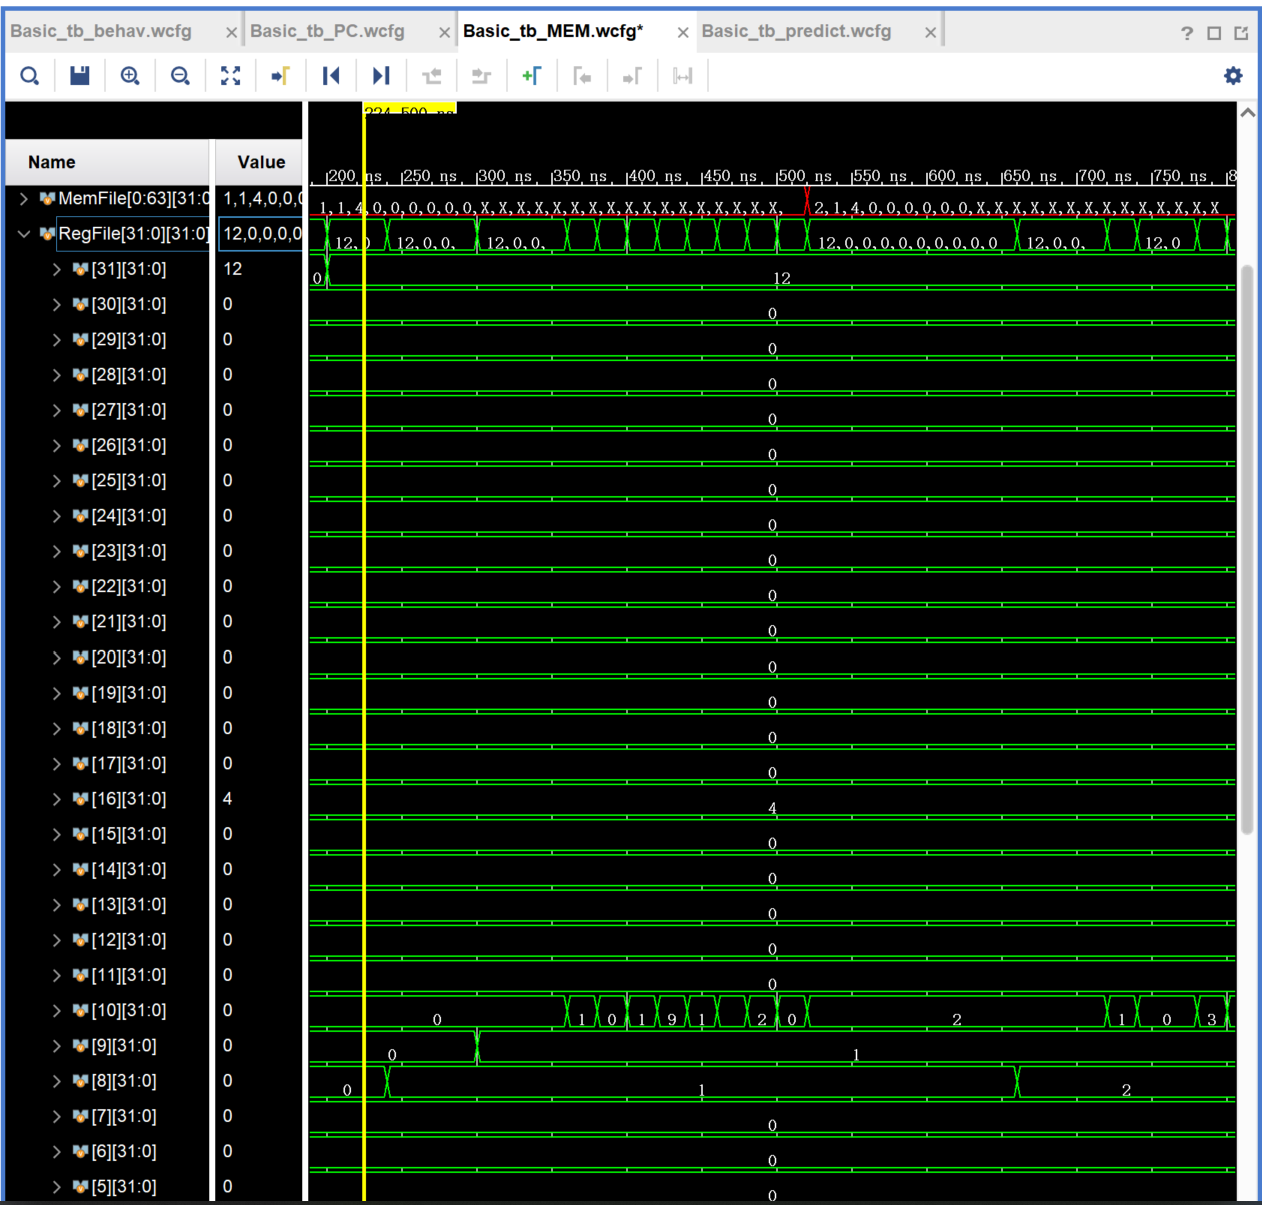
\includegraphics[width=0.5\textwidth]{local.png}
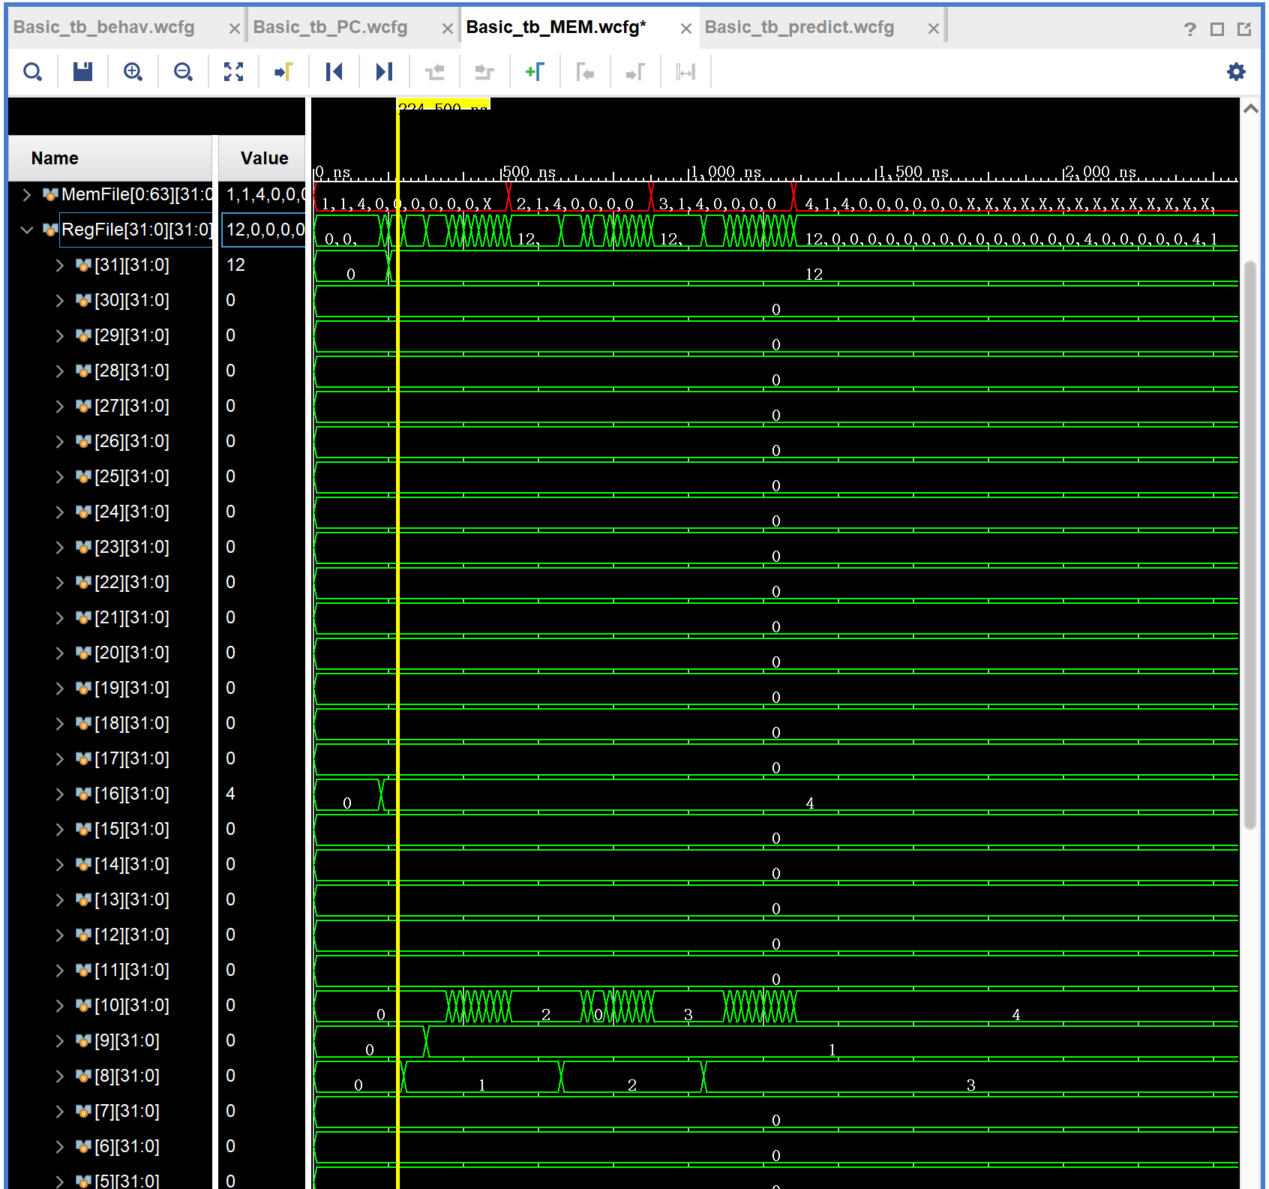
\includegraphics[width=0.5\textwidth]{global.png}

对于前向传递,可以看到由于 ForwardA 被置于 1,ALU第一个输入就会被导入写回数据;由于 ForwardB 被置于 2,ALU第二个输入就会被导入上一个 ALU 的结果。结果如下图所示。该前向传递发生在开始的运算时期,此时的 lw 尚未写回寄存器,但是需要其值。

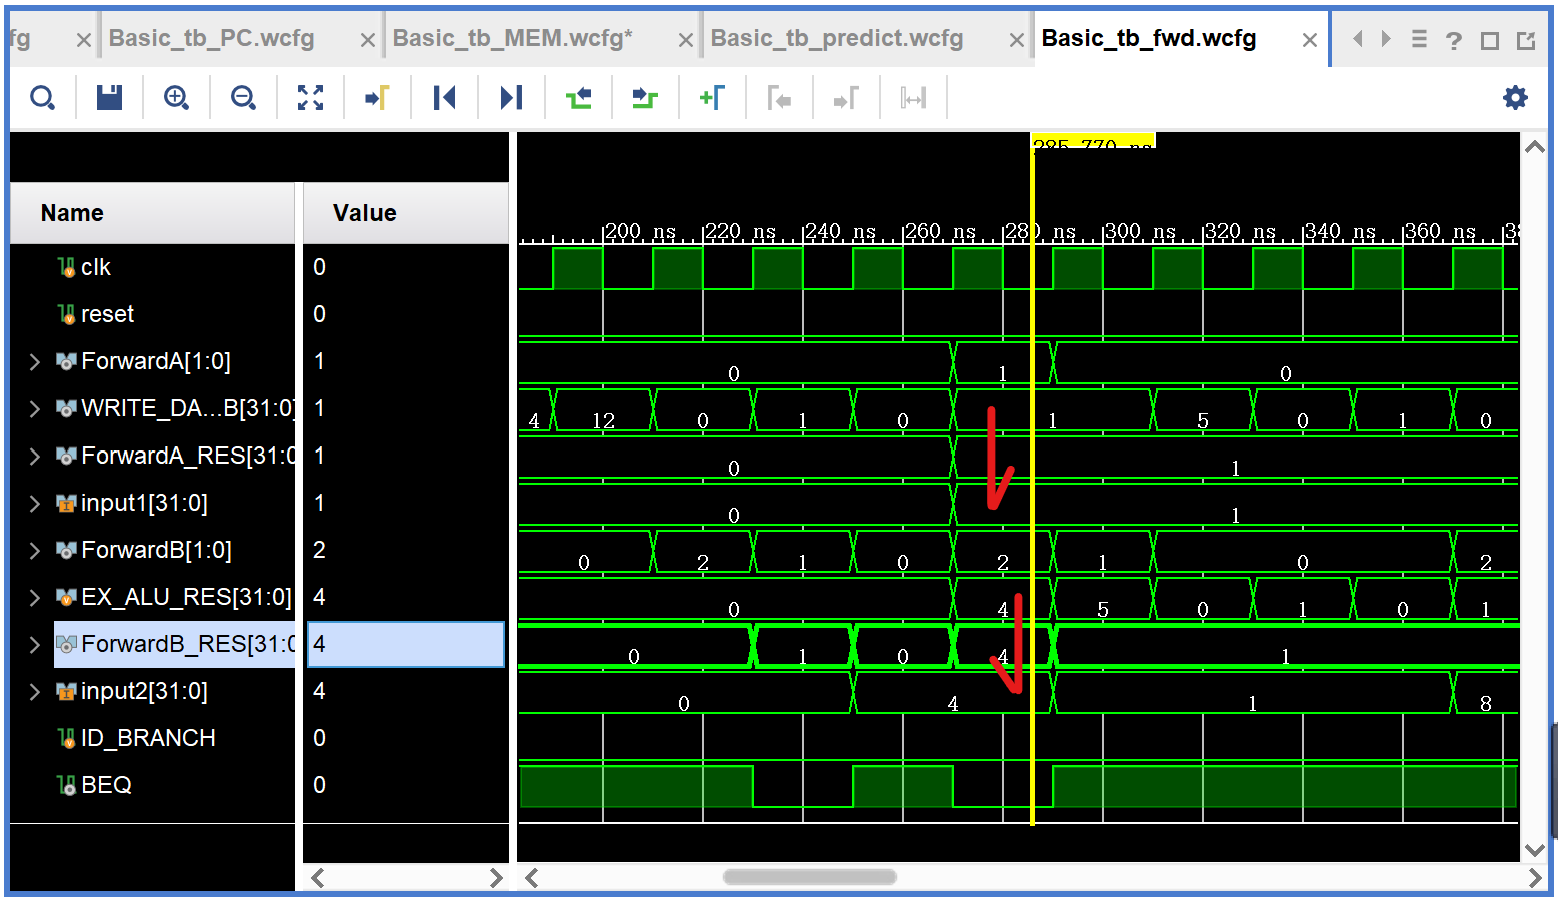
\includegraphics[width=\textwidth]{forward.png}

\subsection{停顿机制}

同一个时期,由于前向传递还不足,就需要停顿一个周期,这个时候 PC 就会被拉长。与此对应的是,所有 ID 控制信号会被清空。

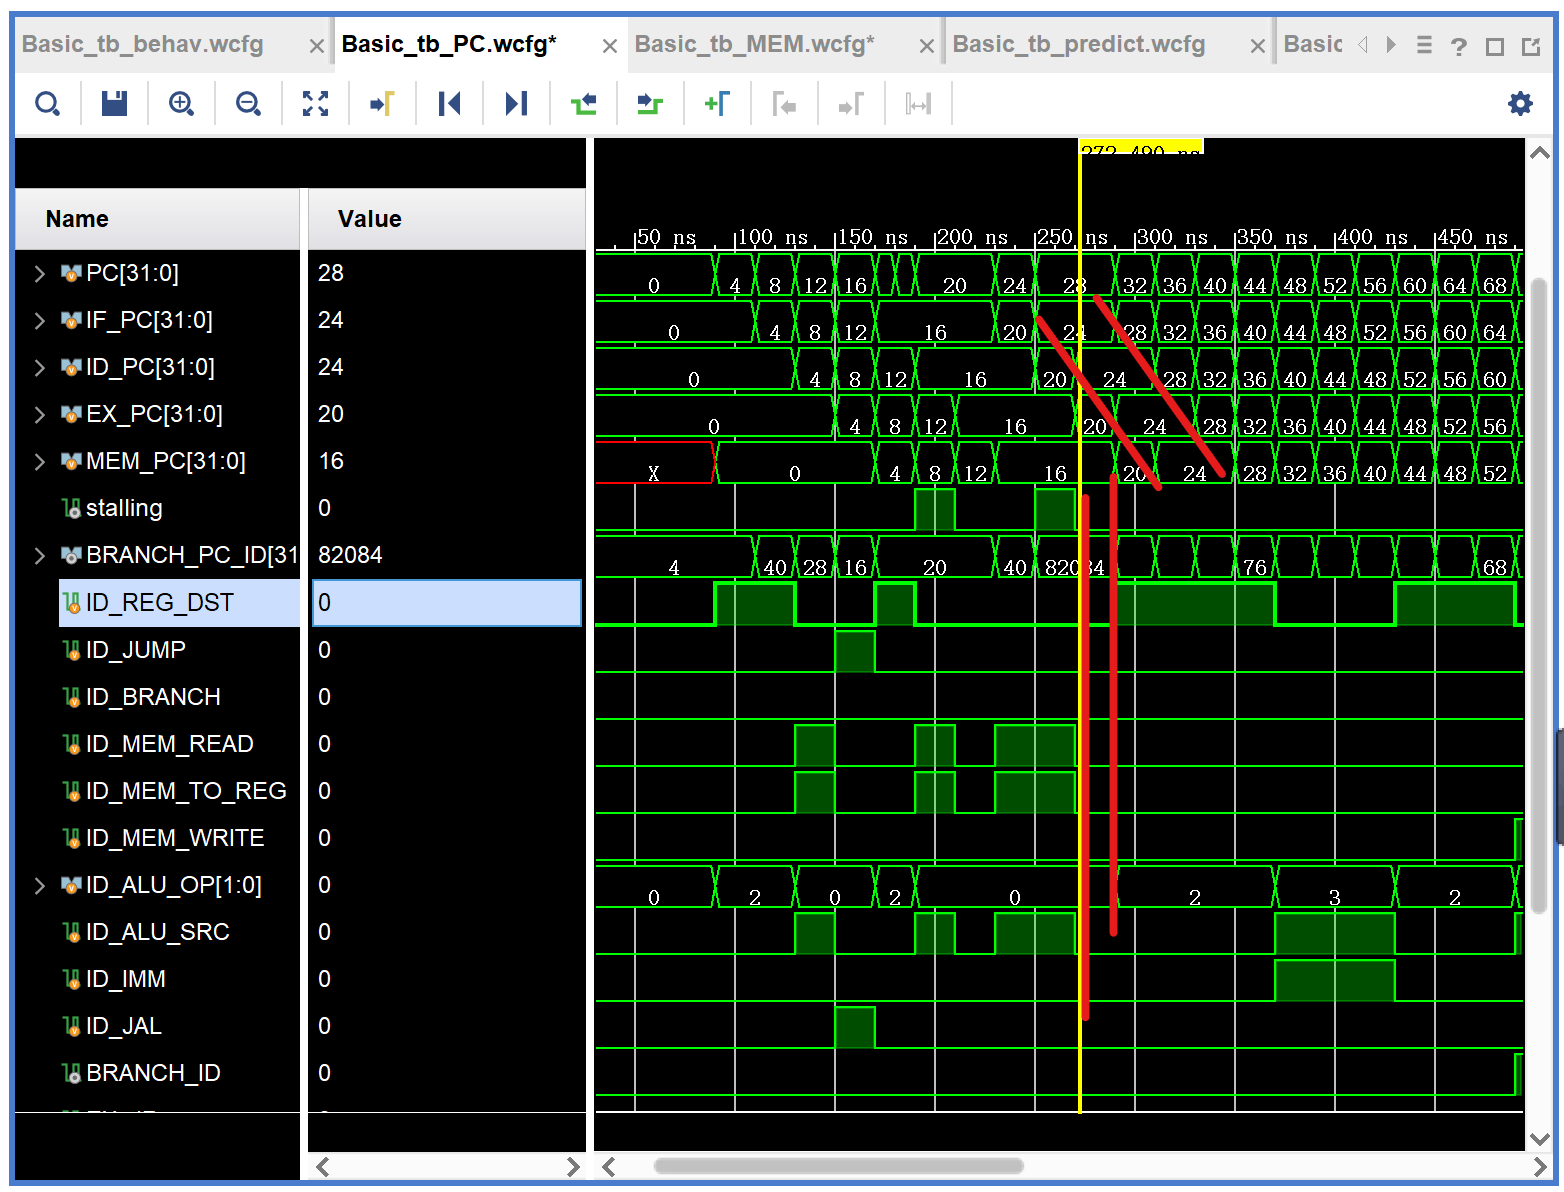
\includegraphics[width=0.8\textwidth]{stalling.png}

\subsection{预测不发生机制}

当最后一个判断时,由于分支发生了,所以将会插入一个气泡,以清除,并且将PC的值进入短循环。

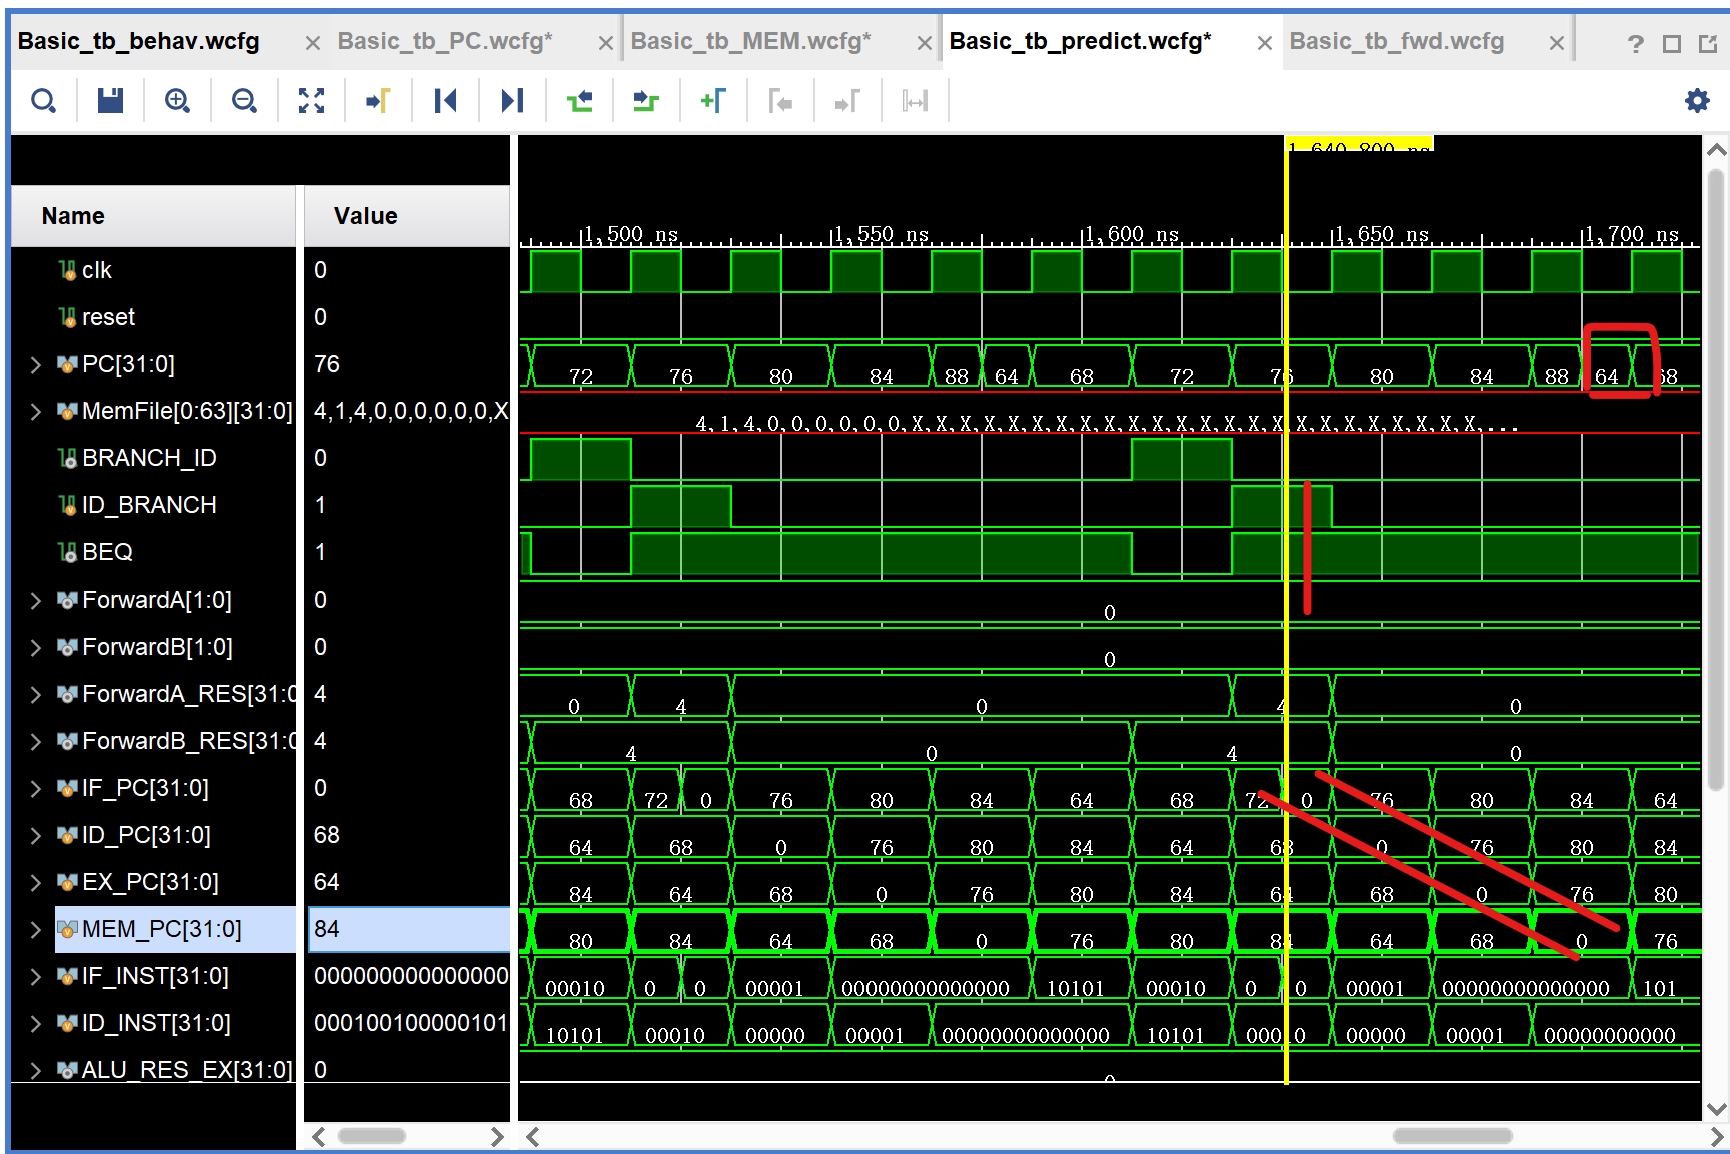
\includegraphics[width=\textwidth]{pnt.png}

\section{实验心得}

计算机系统结构实验终于结束,奋战 4 日的流水处理器终于完成。在设计流水处理器的时候,一直在重新翻看课本,复习概念。在这个过程中加深了我对流水处理器的许多理解。

由于时间不足,所以 31 条指令的选做任务并没有完成,由于需要大改,可能会对代码风格产生影响,并且需要增加很多端口。做完一些减少停顿的策略,理解如何解决冒险足矣。

多次的失败,让我意识到是自己对细节的把握不足,认真看书,总是可以找到对应的答案。感谢实验组给我这个设计处理器的机会,该实验对于我理解处理器的核心细节有很大的帮助。

灵活使用课上的知识,可以更好的解决问题,提高效率(比如使用 Mars 汇编程序)。形成良好的代码风格有助于减少问题发生的几率。并且在无法调试出问题时,不妨建立最小工作集,新建波形,通过代码追踪相关端口,以解决问题。

本实验的处理器原理图形来自参考文献的课本。
\begin{thebibliography}{}
    \bibitem[1]{}
    Computer Organization and Design --- The Hardware/Software Interface, David A. Patterson and John L. Hennessy, Fifth Edition, Elsevier Inc., 2014
\end{thebibliography}

\end{document}